\documentclass{astroedu-lab}

\begin{document}

\pagestyle{plain}

\begin{problem}{\huge Лабораторная работа 5.1.3\\\\Эффект Рамзауэра\\\\Выполнил Жданов Елисей Б01-201}

\section{Цель работы:}

1) Исследовать энергетическую зависимость вероятности рассеяния электроном атомами ксенона

2) Определить энергии электронов, при которых наблюдается "просветление" ксенона

3) Оценить размер внешней электронной оболочки ксенона

\section{Оборудование:}

Тиратрон ТГ3-01/1.3Б

Блок-источник питания

Вольметры

Осциллограф

\section{Теоретическая справка}

Рассеяние электрона на атоме можно приближённого рассматривать как рассеяние частицы энергии $E$ на потенциальной яме длины $\ell$ и глубины $U_0$. Уравнение Шрёдингера имеет вид
\[\Psi'' + k^2 \Psi = 0,\]
где вне ямы 
\[k^2 = k_1^2 = \dfrac{2mE}{\hbar^2},\]
а внутри 
\[k^2 = k_2^2 = \dfrac{2m(E+U_0)}{\hbar^2}.\]
Коэффициент прохождения в таком случае равен
\[D = \dfrac{16 k_1^2 k_2^2}{16k_1^2 k_2^2 + 4(k_1^2 - k_2^2)^2\sin^2(k_2\ell)}.\]
Заметим, что коэффициент прохождения имеет ряд максимумов и минимумов. Он максимальнем при
\begin{equation}\label{0}
\sqrt{\dfrac{2m(E+U_0)}{\hbar^2}}\ell = n\pi,~n=1,2,3,\dots
\end{equation}

Качественно эффект Рамзауэра можно объяснить, рассмотрев интерференцию прошедшей и дважды отразившейся от оболочки волн де Бройля. Длины волн вне и внутри атома:
\[\lambda = \dfrac{h}{\sqrt{2mE}},~\lambda_1 = \dfrac{h}{\sqrt{2m(E+U_0)}}.\]
Соответственно условия на первые интерфереционные максимум и минимум 
\begin{equation}\label{1}
2\ell = \dfrac{h}{\sqrt{2m(E_1 + U_0)}},~2\ell = \dfrac{3}{2}\dfrac{h}{\sqrt{2m(E_2 + U_0)}}.
\end{equation}
Исключая из этих соотношений глубину ямы, получим
\begin{equation}\label{2}
\ell = \dfrac{h\sqrt{5}}{\sqrt{32m(E_2 - E_1)}}.
\end{equation}
Глубина ямы при этом равна
\begin{equation}\label{4}
U_0 = \dfrac{4}{5}E_2 - \dfrac{9}{5}E_1.
\end{equation}

\section{Экспериментальная установка}

\begin{figure}[!h]
	\centering
	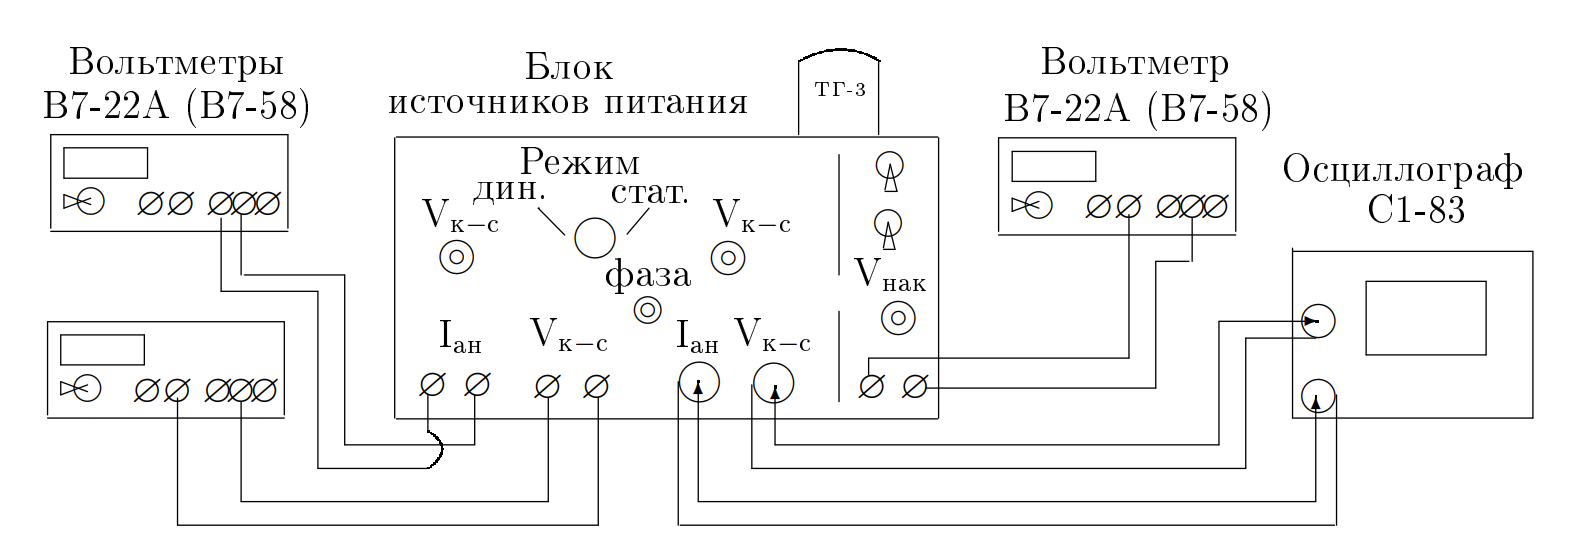
\includegraphics[width=0.9\textwidth]{установка.png}
	\label{fig:boiler}
\end{figure}

Лампа-тиратрон расположена непосредственно на корпусе блока источников питания (БИП), напряжение к электродам лампы подаётся от источников питания, находящихся в корпусе прибора. Регулировка напряжения и выбор режима работы установки производится при помощи ручек управления, выведенных на лицевую панель БИП.


\section{Измерения, Обработка}

%\begin{center}
%\begin{tabular}{|c|c|c|c|}
%\hline 
%\multicolumn{2}{|c|}{$h_\text{ман}$, мм} & $\sigma, \frac{\text{мН}}{\text{К}}$ & T, $^\circ$C \\
%\hline
%188.0 & 188.0 & $(64.5 \pm 3.9)$ & 22\\
%187.0 & 187.0 & $(64.0 \pm 3.9)$ & 30\\
%185.5 & 186.0 & $(63.3 \pm 3.9)$ & 35\\
%184.0 & 184.5 & $(62.5 \pm 3.9)$ & 40\\
%182.5 & 183.0 & $(61.7 \pm 3.9)$ & 45\\
%181.0 & 181.0 & $(60.8 \pm 3.8)$ & 50\\
%179.0 & 179.5 & $(59.9 \pm 3.8)$ & 55\\
%177.5 & 177.5 & $(59.0 \pm 3.8)$ & 60\\
%\hline
%\end{tabular}
%\end{center}

\subsection{Динамический режим}

С помощью осциллографа снимаем ВАХ в динамическом режиме при двух различных напряжениях накала.

Погрешность напряжения возьмем $\sigma_U = 0.01~\text{В}$, соответствующую его случайным колебаниям в процессе измерений.

По ВАХ определим $V_{\text{max}}$, $V_{\text{min}}$ и $V_{\text{пробой}}$ (см. таблицу ниже). Погрешности всех проведенных на осциллографе измерений -- $\sigma_V = 0.3~\text{В}$ -- цена деления, умноженная на $\sqrt{2}$, так как точки на двух кривых неточно совпадали по своему положению.

\begin{center}
	
\end{center}

\begin{table}[h]
\begin{tabular}{|c|c|c|c|c|c|c|}
\hline
  & $U$, В & $V_{\text{max}}$, В & $V_{\text{min}}$, В & $V_{\text{пробой}}$, В \\ \hline
1 & $2.60  \pm  0.01$          & $1.6 \pm 0.4$                   & $6.2 \pm 0.4$                 & $11.4 \pm 0.4$                        \\ \hline
2 & $2.97   \pm 0.01$          & $1.8 \pm 0.4$                   & $5.2 \pm 0.4$                 & $11.2 \pm 0.4$                   \\ \hline
\end{tabular}
\centering
\caption{Измерения по ВАХ тиратрона}
\end{table}

Проверим рассчёт $\ell$ по формулам \eqref{1} на предмет того, яма меньше предполагаемых $U_0 = 2.5~\text{эВ}$ или нет.

Действительно для первого напряжения лампы:

\begin{equation}
	l(1) = \dfrac{h}{\sqrt{2m(V_{max} + U_0)}} = 3.03 \pm 0.16 \text{ A}
\end{equation}

\begin{equation}
	l(2) = \dfrac{h}{\sqrt{2m(V_{min} + U_0)}} = 3.12 \pm 0.08 \text{ A}
\end{equation}

Для второго:

\begin{equation}
	l(1) = \dfrac{h}{\sqrt{2m(V_{max} + U_0)}} = 2.96 \pm 0.15 \text{ A}
\end{equation}

\begin{equation}
	l(2) = \dfrac{h}{\sqrt{2m(V_{min} + U_0)}} = 3.32 \pm 0.09 \text{ A}
\end{equation}

Также найдём $\ell$ и глубину ямы по формулам \eqref{2} и \eqref{4}:


\[\ell(U_\text{нак} = 2.6 \text{В}) = \dfrac{h\sqrt{5}}{\sqrt{32m(E_2 - E_1)}} = 3.20 \pm 0.3 \text{ A}  \]

\[\ell(U_\text{нак} = 2.6 \text{В}) = \dfrac{h\sqrt{5}}{\sqrt{32m(E_2 - E_1)}} = 3.70 \pm 0.5 \text{ A}  \]

\[U_0(U_\text{нак} = 2.6 \text{В}) = 2.1 \pm 1.0~\text{эВ}.\]

\[U_0(U_\text{нак} = 2.97 \text{В}) = 0.9 \pm 1.0~\text{эВ}.\]

Усредним значения и получим результат

\[U_0 = 1.5 \pm 0.8~\text{эВ}.\]

\[\ell = 3.5 \pm 0.3 \text{ A} \]

Погрешности посчитаны на основании абсолютных и статистической погрешностей величин.

С теоретическими значениями $\ell = 2.8 \text{ A}$ и $U_0 = 2.5 \text{  В} $ полученные величины сходятся в рамках погрешностей, хотя и заметно отличаются.


Оценим ионизационный потенциал как 
\[U = U_0 + V_{\text{пробой}} = 12.8 \pm 1.2~\text{эВ}.\]
Сравнивая с потенциалами ионизации, приведёнными в описании работы, видим, что полученный потенциал в пределах погрешности совпадает с ионизационным потенциалом ксенона $U = 12.1~\text{эВ}$.\\

\subsection{Статический режим}

Теперь снимем ВАХ титратрона в статическом режиме при тех же значениях напряжения накала, представим данные в виде графиков ниже. Проведя аналогичные расчёты, получим:

\begin{table}[h]
\begin{tabular}{|c|c|c|c|c|c|c|}
\hline
  & $U$, В & $V_{\text{max}}$, В & $V_{\text{min}}$, В & $V_{\text{пробой}}$, В \\ \hline
1 & $2.60  \pm  0.01$          & $1.6 \pm 0.2$                   & $6.0 \pm 0.5$                 & $11.5 \pm 0.5$                        \\ \hline
2 & $2.97   \pm 0.01$          & $1.7 \pm 0.2$                   & $5.2 \pm 0.5$                 & $11 \pm 1$                   \\ \hline
\end{tabular}
\centering
\caption{Измерения по ВАХ тиратрона}
\end{table}

\[\ell = 3.4 \pm 0.3 A\]
\[U_0 = 1.4 \pm 0.5~\text{эВ}.\]

График ниже был предварительно усреднен, а погрешность оценена таким образом: показания тока плыли на характерные 5 мкА за время подстройки напряжения. Фактически такие кресты погрешности будут у точек графика. Обозначим погрешность размерном точек. Характерная погрешность по напряжению окажется 0.5 Вольт у минимума и 0.2 Вольт у максимума.

Из формулы \eqref{0} оценим значения напряжений максимумов порядка $n > 2$:
\[E_2 = 20.41~\text{эВ},~E_2 = 47.61~\text{эВ},~E_4 = 85.69~\text{эВ}.\]

Полученные энергии выше потенциала ионизации, поэтому эти максимумы уже не будут наблюдаться.
\begin{figure}[h]
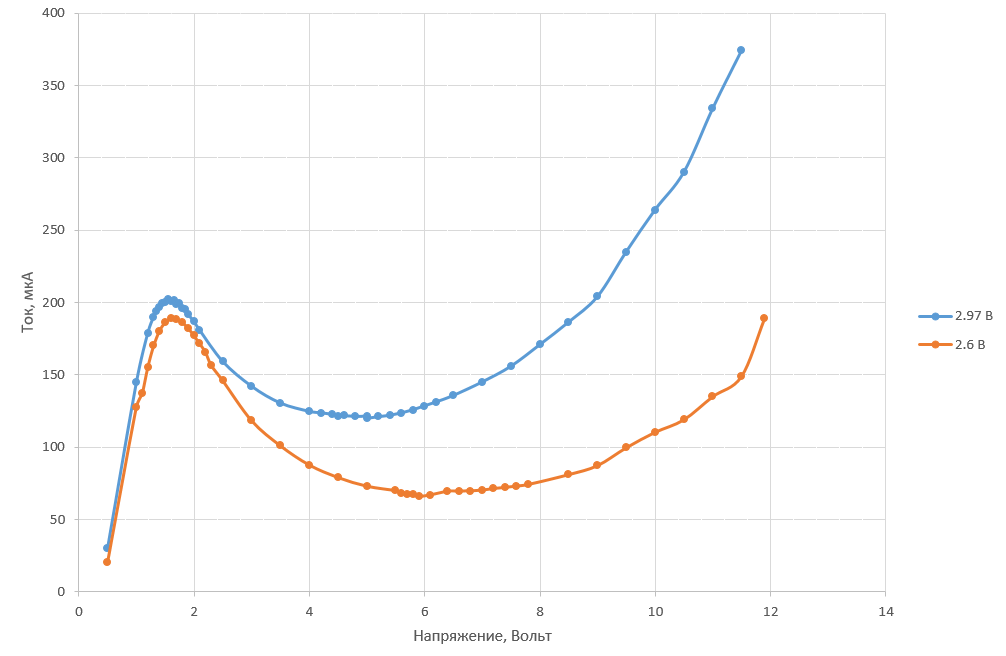
\includegraphics[width=0.7\textwidth]{граф.png}
\centering
\caption{ВАХ титратрона при разных напряжениях накала.}
\end{figure}

\newpage

Наконец, можно получит зависимость вероятности рассеяния от напряжения на титротроне. Качественный график приведён на рисунке(поскольку ток катода неизвестен и зависит от напряжения на лампочке) 

\begin{figure}
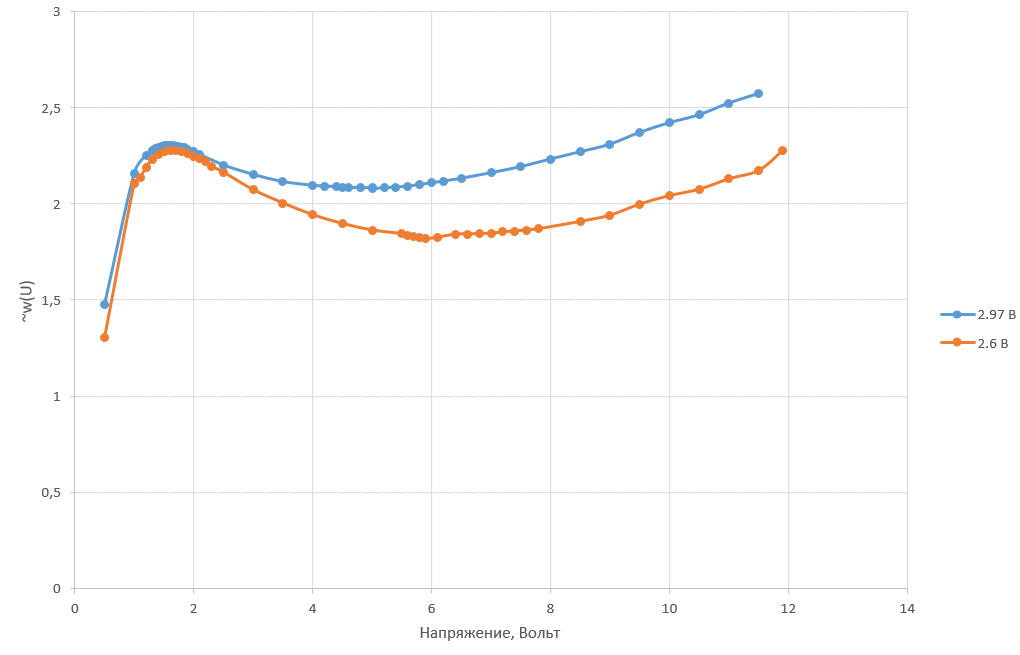
\includegraphics[width = 0.7\textwidth]{wu.png}
\centering
\caption{Качественный вид зависимости $w = w(V)$.}
\end{figure}


\section{Вывод}

Полученные значения, хоть и близки к теоретическим, оказались немного заниженными. 

Тем не менее, эксперимент прекрасно подтверждает сам эффект Рамзауэра, на вольт амперных характеристиках отчетливо видны пики максимума и минимума поглощения. 

Подведем вывод по полученным значениям:
\\
\begin{table}[h]
\begin{tabular}{|c|c|c|c|}
\hline
  & Энергия ионизации, эВ & $U_0$ В & $\ell$, А \\ \hline
Теоретически & 12.1 & 2.5 & 2.8  \\
Динамика & $12.8 \pm 1.2$       & $1.7 \pm 0.2$                   & $3.5 \pm 0.3$                               \\
Статика & $12.9 \pm 1.0$      & $1.4 \pm 0.5$                   & $3.4 \pm 0.3$                                  \\ \hline
\end{tabular}
\centering
\caption{Результаты}
\end{table}

Принципиальной разницы в точности статического и динамического метода не было обнаружено, что в очередной раз подчеркивает, что оборудование было хорошо откалибровано, и все значения корректные.

Вероятностное распределение также зависит от напряжения согласованно с теорией.

Итак, все цели работы выполнены.


\end{problem}
\end{document}